%\begin{listing}[]
\begin{minipage}{.5\textwidth}
\begin{minted}
[
fontsize=\scriptsize,
linenos=true,
escapeinside=||,
breaklines
]
{go}
package main
import "sync"

type Container struct{ |\label{bugListing:containerType_start}|
  sync.Mutex
  stop  chan struct{}
} |\label{bugListing:containerType_end}|

func main() {
  container := &Container{ |\label{bugListing:container_create_start}|
       stop:make(chan struct{})} |\label{bugListing:container_create_end}|
  go Monitor(container) |\label{bugListing:main_go_monitor}|
  go StatusChange(container) |\label{bugListing:main_go_statChange}|
}
\end{minted}
\end{minipage}
\begin{minipage}{.35\textwidth}
\begin{minted}
[
fontsize=\scriptsize,
linenos=true,
escapeinside=||,
breaklines
]
{go}
|\setcounter{FancyVerbLine}{15}|func Monitor(cnt *Container){
  for{
    select{
    case <- cnt.stop:  |\label{bugListing:Monitor_case_recv}|
      return |\label{bugListing:Monitor_case_recv_ret}|
    default: |\label{bugListing:Monitor_case_def}|
      cnt.Lock()  |\label{bugListing:Monitor_case_def_lock}|
      cnt.Unlock() |\label{bugListing:Monitor_case_def_unlock}|
}}}
func StatusChange(cnt *Container){
  cnt.Lock() |\label{bugListing:statChange_lock}|
  cnt.stop <- struct{}{} |\label{bugListing:statChange_send}|
  cnt.Unlock() |\label{bugListing:statChange_defer_unlock}|
}
\end{minted}
\end{minipage}
\begin{minipage}{.29\textwidth}
  \centering
  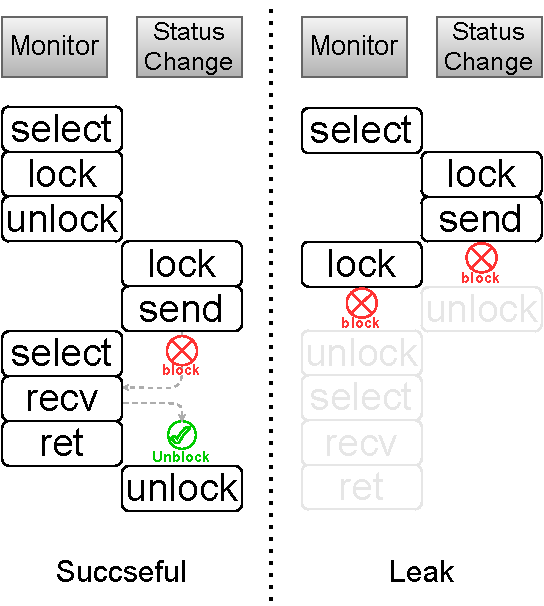
\includegraphics[width=.99\linewidth]{figs/execViz_moby.pdf}
\end{minipage}
\caption{Simplified version of bug \texttt{moby28462}}
\label{listing:moby28462}
\end{listing}

\begin{listing*}[]
\begin{minipage}{.35\textwidth}
\begin{minted}
[
fontsize=\footnotesize,
linenos=true,
escapeinside=||,
breaklines
]
{go}
package main
import "sync"

type Container struct{ |\label{bugListing:containerType_start}|
  sync.Mutex
  stop  chan struct{}
} |\label{bugListing:containerType_end}|

func main() {
  container := &Container{ |\label{bugListing:container_create_start}|
       stop:make(chan struct{})} |\label{bugListing:container_create_end}|
  go Monitor(container) |\label{bugListing:main_go_monitor}|
  go StatusChange(container) |\label{bugListing:main_go_statChange}|
}
\end{minted}
\end{minipage}
\begin{minipage}{.35\textwidth}
\begin{minted}
[
fontsize=\scriptsize,
linenos=true,
escapeinside=||,
breaklines
]
{go}
|\setcounter{FancyVerbLine}{15}|func Monitor(cnt *Container){
  for{
    select{|\label{bugListing:Monitor_select}|
    case <- cnt.stop:  |\label{bugListing:Monitor_case_recv}|
      return |\label{bugListing:Monitor_case_recv_ret}|
    default: |\label{bugListing:Monitor_case_def}|
      cnt.Lock()  |\label{bugListing:Monitor_case_def_lock}|
      cnt.Unlock() |\label{bugListing:Monitor_case_def_unlock}|
}}}
func StatusChange(cnt *Container){
  cnt.Lock() |\label{bugListing:statChange_lock}|
  defer cnt.Unlock() |\label{bugListing:statChange_defer_unlock}|
  cnt.stop <- struct{}{} |\label{bugListing:statChange_send}|
}
\end{minted}
\end{minipage}
\begin{minipage}{.25\textwidth}
  \centering
  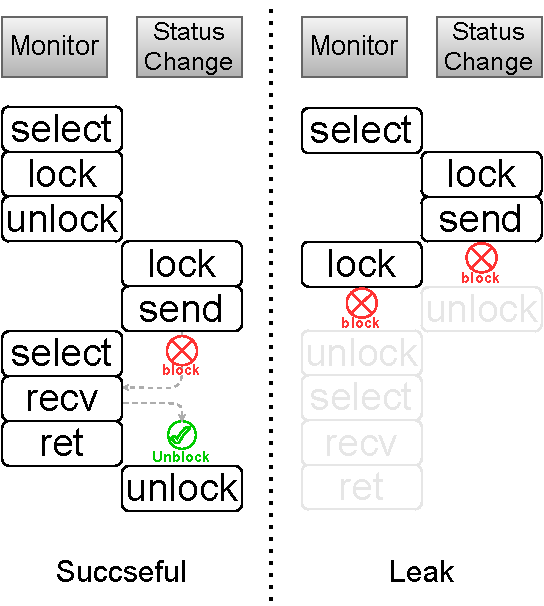
\includegraphics[width=.99\linewidth]{figs/execViz_moby.pdf}
\end{minipage}
\caption{Simplified version of bug \texttt{moby28462}}
\label{listing:moby28462.minipage}
\end{listing*}

%\begin{listing}[]
\begin{minipage}{.45\columnwidth}
\begin{minted}
[
fontsize=\footnotesize,
linenos=true,
escapeinside=||,
xleftmargin=2em,
breaklines
]
{go}
package main
import "sync"

type Cont struct{|\label{bugListing:containerType_start}|
  sync.Mutex
  stop  chan struct{}
}|\label{bugListing:containerType_end}|

func main() {
  cnt := &Cont{|\label{bugListing:container_create_start}|
       stop:make(chan struct{})}|\label{bugListing:container_create_end}|
  go Monitor(cnt)|\label{bugListing:main_go_monitor}|
  go StatusChange(cnt)|\label{bugListing:main_go_statChange}|
}
\end{minted}
\end{minipage}\hfill
\begin{minipage}{.45\columnwidth}
\begin{minted}
[
fontsize=\footnotesize,
linenos=true,
escapeinside=||,
breaklines
]
{go}
|\setcounter{FancyVerbLine}{15}|func Monitor(cnt *Cont){
  for{
    select{
    case <- cnt.stop:  |\label{bugListing:Monitor_case_recv}|
      return |\label{bugListing:Monitor_case_recv_ret}|
    default: |\label{bugListing:Monitor_case_def}|
      cnt.Lock()  |\label{bugListing:Monitor_case_def_lock}|
      cnt.Unlock() |\label{bugListing:Monitor_case_def_unlock}|
}}}
func StatusChange(cnt *Cont){
  cnt.Lock() |\label{bugListing:statChange_lock}|
  defer cnt.Unlock() |\label{bugListing:statChange_defer_unlock}|
  cnt.stop <- struct{}{} |\label{bugListing:statChange_send}|
}
\end{minted}
\end{minipage}
\caption{Simplified version of bug \texttt{moby28462}}
\label{listing:moby28462}
\end{listing}


\subsection{Go Concurrency}
\label{sec:goConcurrency}
%
Go introduces a new concurrency model, mixing shared-memory features of languages like Java/C/C++ and message-passing concepts such as Erlang's, with an ad-hoc scheduler that orchestrates Go's concurrent components interactions while shielding the user from many low-level aspects of the runtime.
%
The language is equipped with a rich vocabulary of \textit{serialization} features to facilitate the memory model constraints~\cite{go-memModel}; they include synchronous and asynchronous communication, memory protection, and barriers for efficient synchronization:
\begin{itemize}
    \item \textbf{Goroutines} are functions that execute concurrently on logical processors having their own stack.
    \item \textbf{Channels} are typed conduits through which goroutines communicate.  Channels are unbuffered by default, providing synchronous (rendezvous) or asynchronous (via buffered channels) messaging between goroutines.
    \item \textbf{Synchronization} features such as \textit{(RW)mutex}, \textit{waitGroup}, \textit{conditional variables}, \textit{select}, and \textit{context} are included in the language to provide more and flexible synchronization, data access serialization, memory protection, and error handling.
    \item \textbf{Scheduler} maintains goroutines in FIFO queues and binds them on OS threads to execute on processing cores.
\end{itemize}


This design facilitates the construction of data flow models that efficiently utilize multiple CPU cores and encourages developers to \textit{share memory through communication} for safe and straightforward concurrency and parallelism.
%
This rich mixture of features has, unfortunately, greatly exacerbated the complexity of debugging.
%
In fact, the popularity of Go has outpaced its debugging support~\cite{go-survey,tu-concurrentBugs-asplos19,yuan-gobench-cgo21}.
%
There are some encouraging developments in support of debugging, such as a data race checker \cite{go-race-blog} that has now become a standard feature of Go, and has helped catch many a bug.
%
However, the support for blocking bugs such as deadlocks and Go-specific bug-hunting support for Go idioms (e.g., misuse of channels and locks) remain insufficiently addressed.




%\stcmtside{Explaining the example to motivate}
Listing \ref{listing:moby28462.minipage} shows a simplified version of a reported bug in Docker \cite{moby-28462-commit}.
%
An instance of the \texttt{Container} type (lines \ref{bugListing:containerType_start}-\ref{bugListing:containerType_end}) is created in the \texttt{main} function (lines \ref{bugListing:container_create_start}-\ref{bugListing:container_create_end}).
%
In line \ref{bugListing:main_go_monitor}, a goroutine is spawned to execute function \texttt{Monitor} that continuously checks the container status and returns once it receives from the container's channel (lines \ref{bugListing:Monitor_case_recv}-\ref{bugListing:Monitor_case_recv_ret}).
%
The default case of the \texttt{select} statement (line \ref{bugListing:Monitor_case_def}) allows \texttt{Monitor} to continue monitoring without getting blocked on the channel receive (line \ref{bugListing:Monitor_case_recv}).
%
Concurrent to the \texttt{main} and \texttt{Monitor} goroutines, another goroutine is created in line  \ref{bugListing:main_go_statChange} to execute function \texttt{StatusChange} which changes the status of the container by sending to the container's channel.
%
The container's lock is released after the send action completes and function returns (\texttt{defer} statement in line \ref{bugListing:statChange_defer_unlock}).
%


Native execution of this program terminates successfully without issuing any error or warning.
%
Based on the Go specification and memory model, there is no constraint on the goroutines spawned from the \texttt{main} function to join back before the \texttt{main} goroutine\footnote{In the remainder of the paper, we use \textit{main function} and \textit{main goroutine} interchangeably.} terminates.
%
A deadlock detector within the runtime periodically checks that the scheduler queues of all \textit{runnable} goroutines never become empty until the \texttt{main} goroutine terminates.
%
In other words, the runtime throws a deadlock exception when the \texttt{main} goroutine is blocked, and no other goroutine is in the queue to execute (\ie \textit{global deadlock}).
%
Since there is no blocking instruction in the \texttt{main} goroutine in listing \ref{listing:moby28462.minipage}, the program terminates successfully regardless of other goroutines' statuses.
%
However, this program suffers from a common bug in concurrent Go where one or more goroutines \textit{leak} (\ie \textit{partial deadlock}) from the execution (\ie never reach their end states).

%\stcmtside{Explain the deadlock (leak) situation that might get overlooked}
%Due to the non-determinism introduced by the runtime scheduler and application-level random features like \texttt{select}, many interleavings are feasible for concurrent execution of simple programs such as listing \ref{listing:moby28462.minipage}.
%
The right side of the listing displays a successful run and a leak situation of the program.
%
In the leak situation, first, the \texttt{Monitor} goroutine executes the \texttt{select} statement and, based on the available cases, picks the default case to execute.
%
Right before the execution of mutex lock (line \ref{bugListing:Monitor_case_def_lock}), the scheduler context-switches and the \texttt{StatusChange} goroutine starts its execution through which it holds the lock and blocks on sending to the channel (line \ref{bugListing:statChange_send}) since there is no receiver on that channel.
%
Upon blocking on send, the scheduler transfers back the control to the \texttt{Monitor} goroutine that tends to acquire the mutex, but because the mutex is already held by \texttt{StatusChange}, the \texttt{Monitor} goroutine also blocks.
%
The circular wait between the container mutex and channel prevents both spawned goroutines from reaching their end states and leaves the program in an unnoticed deadlock situation.
%
%\stcmtside{The thirst for novel and scalable debuggers}
%Widely used deadlock detectors such as Goodlock \cite{havelund-goodlock-spin00} are not applicable in Go since causes of Go deadlocks are resources (\eg locking a locked mutex) or communication (\eg sending on a full channel), or a combination of them (\eg leaky interleaving of listing \ref{listing:moby28462.minipage}).
%
%In addition, due to the light-weight nature of goroutines, it is not uncommon to spawn thousands of goroutines in production software systems.
%
%Hence,  novel and scalable techniques are needed to enable realistic modeling of program behavior during execution.
%


\subsection{Concurrency Bugs in Go}
\label{sec:goBugs}
Based on a proposed bug taxonomy for Go \cite{tu-concurrentBugs-asplos19}, bugs are categorized separately based on their \textit{causes} (shared-memory vs. message-passing) and \textit{symptoms} (blocking vs. non-blocking).
%
Blocking bugs historically refer to situations where one or more processing units (\eg goroutines) are blocked, waiting for an external signal to resume (\eg leak situation in listing \ref{listing:moby28462.minipage}.
%
The observed causes of such blocking flaw in the context of Go are as follows:

\begin{itemize}
  \item \textit{Resource deadlocks}: Go inherits resource deadlocks from multithreaded languages like Java and C/Pthreads where goroutines are trapped in a circular wait for the resource (\eg mutex) that is held by other goroutines.
  \item \textit{Communication deadlocks}: Synchronized (unbuffered) channels transmit values from one goroutine to another in a rendezvous fashion. The sender (or receiver) blocks until the receiver (or sender) is ready to receive (send). Misuse of channel operations might result in one or more goroutines waiting for a sender/receiver to unblock them forever.
  \item \textit{Mixed deadlocks}: The leak situation in listing \ref{listing:moby28462.minipage} is the example of such deadlocks where one goroutine is blocked on acquiring a resource that is held by another goroutine which is blocked on communication.
\end{itemize}
\stcmtside{about race}
Go inherited traditional non-blocking bugs such as data races and atomicity violations from older concurrent languages while introducing new bug idioms due to its new concepts such as anonymous functions \cite{tu-concurrentBugs-asplos19}.
%

\noindent{\bf Application-level non-determinism:\/}
In addition to the non-deterministic nature of concurrent languages caused by the scheduler and interaction between concurrent components, Go introduces some level of non-determinism at the application level.
%
The \textit{select-case} statement (similar to switch-case) allows the goroutine to wait on multiple channel operations.
%
Go runtime picks one case pseudo-randomly among available cases of selects (\ie channel sends and receives that are ready to execute without blocking).
%
If none of the cases are ready, the executing goroutine is blocked unless there is a \textit{default} case.
%
The default case makes the select non-blocking and prevents the goroutine from waiting for unavailable communications.
%
Such random behavior expands the schedule-space exploration, especially when select statements are used in nested fashion within nested loops.
%
Hence, root-causing the misbehaved execution of a buggy program becomes more challenging.
%
Our experiments/observations (section or table \ref{} **FIXME**) demonstrate that select statements are in the core of rare bugs.


\subsection{Execution Concurrency Tracing (ECT)}
\label{sec:ect}
The primary cause of most real-world concurrent bugs is the misuse of concurrency features like channels, mutexes, and waitGroups (table \ref{tab:comparison}).
%
To gain insight into the behavior of concurrency features during execution, we equipped \goat with a tracing mechanism~\cite{ect-arxiv}, which is an extension to the Go built-in tracer package~\cite{go-cmd-trace}.
%
The tracing capability is compiled into all programs always through the runtime and is enabled on demand -- when tracing is disabled, it has minimal runtime overhead \cite{go-exec-tracer-doc}.
%
%We chose the tracer package to enhance because it 1) is already compiled into the runtime, 2) adds minimal overhead, and 3) only lacks some pieces allowing the construction of an accurate concurrency model.
%

\textit{Execution concurrency trace} (ECT) is a totally ordered \textit{sequence} of events in which the order is approximated through a central clock with nanosecond precision.
%
ECT also contains the call-stack for each event, enabling a direct mapping of events to source-line numbers.
%
The alphabet of ECT is total of 63 events -- 49 from original tracer package \cite{goParserSource}, categorized and summarized in table \ref{tab:events} and 14 additional events that we added to capture concurrency usage events:
%
\begin{itemize}
    \item \textbf{Channel:} For each channel operation (make, send, receive, close), ECT includes an event with a unique id assigned to each channel.
    \item \textbf{(RW)Mutex, WaitGroup \& Conditional Variables:} Similar to channels, we assign a unique id to each concurrency object and emit an event for each of their operations (lock, unlock, rlock, runlock, add, wait, signal, broadcast).
    \item \textbf{Select \& Schedule:} The scheduler and the \textit{select} structure introduce non-determinism to the execution. We keep track of the decisions made by the scheduler and select statements to obtain an accurate decision path during execution.
\end{itemize}

%\stcmtside{how ECT captures concurrency blocking behavior}


%
For each blocking operation (channels \textit{sends}/\textit{recvs}, mutex \textit{locks}, waitGroup/conditional variable \textit{wait} and \textit{select} (when none of the cases are available)), ECT captures a pair of pre-operation and post-operation events to distinguish between the \textit{request for action} and \textit{completion of action}.
%
Hence, ECT is especially effective for debugging because it enables modeling the blocking state of program execution at any given step of execution.
%
More details about the implementation of trace package enhancement and scalability report are available in \cite{ect-arxiv}

\begin{table}[]
    \centering
        \begin{tabular}{|l|l|}
        \hline
        \rowcolor[HTML]{C0C0C0}
        \multicolumn{1}{|c|}{\cellcolor[HTML]{C0C0C0}\textbf{Category}} & \multicolumn{1}{c|}{\cellcolor[HTML]{C0C0C0}\textbf{Description}} \\ \hline
        Process & Indication of process/thread start and stop \\ \hline
        GC/Mem & Garbage collection and memory operation events\\ \hline
        Goroutine & Goroutines events: create, block, start, stop, end, etc. \\ \hline
        Syscall & Interactions with system calls \\ \hline
        Users & User annotated regions and tasks (for bounded tracing) \\ \hline
        Misc & System related events like futile wakeup or timers \\ \hline
        \end{tabular}

    \caption{Event categories by the Go execution tracer}
    \label{tab:events}
\end{table}
